\chapter{Maxwell-Gleichungen, Kovarianz und elektromagnetische Wellen}

\lectureoverview{Elektrische und magnetische Felder üben über die Lorentzkraft Kräfte auf geladene Materie aus, doch Materie muss auch die Felder erzeugen und umverteilen. Wir formulieren diese wechselseitige Seite des Elektromagnetismus, zeigen, dass die Maxwell-Gleichungen Lorentz-kovariant sind, leiten ihre Well Lösungen her und führen anschließend Ladung und Strom in einer Form wieder ein, in der die lokale Erhaltung unmittelbar sichtbar ist. In der gesamten Vorlesung verwenden wir Einheiten, in denen \(c=1\) gilt.}

\section{Die andere Seite des Elektromagnetismus}

Beginnen wir mit dem Teil des Themas, den wir bereits behandelt haben. Bewegt sich ein Teilchen mit der Ladung \(q\) und der Geschwindigkeit \(\mathbf v\) durch elektrische und magnetische Felder, so wirkt auf es die Kraft
\begin{equation}
\mathbf F=q\bigl(\mathbf E+\mathbf v\times\mathbf B\bigr).
\label{eq:lorentz-force-three}
\end{equation}
Der Faktor \(q\) ist unverzichtbar. Ein ungeladenes Teilchen erfährt keine elektromagnetische Kraft. Der elektrische Beitrag wirkt auch dann, wenn das Teilchen momentan in Ruhe ist, während der magnetische Beitrag von seiner Bewegung abhängt.

Gleichung~\eqref{eq:lorentz-force-three} sagt uns, wie vorgegebene Felder auf Materie wirken. Sie sagt uns nicht, wodurch die Felder bestimmt werden. Was erzeugt ein elektrisches Feld um einen Gegenstand, ein magnetisches Feld um einen anderen oder eine Welle, die sich durch den leeren Raum bewegt? Die Gleichungen, die diese Fragen beantworten, sind die Maxwell-Gleichungen.

\begin{figure}[H]
\centering
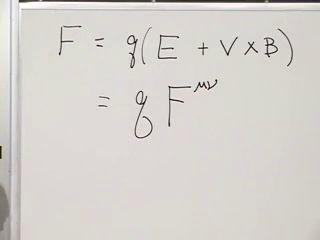
\includegraphics[width=0.62\textwidth]{lecture_58_figure_02.png}
\caption{Die Lorentzkraft als Dreivektorgleichung und der Beginn ihrer tensorielle Umformulierung.}
\lectureframe{00:05:49}
\end{figure}

Die relativistische Form des Kraftgesetzes führt die Notation ein, die wir benötigen werden:
\begin{equation}
f^\mu=qF^\mu{}_{\nu}u^\nu.
\label{eq:lorentz-force-four}
\end{equation}
Hier ist \(u^\nu\) die Vierergeschwindigkeit, \(f^\mu\) die Viererkraft und \(F^{\mu\nu}\) ein antisymmetrischer Tensor, der aus \(\mathbf E\) und \(\mathbf B\) zusammengesetzt ist. Auf der Tafel ist zunächst nur der schematische Anfang dieses Ausdrucks zu sehen; die Kontraktion mit \(u^\nu\) liefert den fehlenden Vektor, sodass ein Kraftindex frei bleibt.

Es gibt einen physikalischen Grund dafür, dass Materie auf das Feld zurückwirken muss. Eine elektromagnetische Welle kann auf eine Ladung treffen, sie beschleunigen und ihr Energie übertragen. Könnte das Feld auf die Ladung einwirken, während die Ladung niemals auf das Feld einwirken könnte, gäbe es keinen Ort, von dem diese Energie entzogen würde. Wirkung und Gegenwirkung sind nicht das ganze Argument, aber die Energieerhaltung macht die wechselseitige Kopplung unvermeidlich.

\section{Eine sich ändernde Quelle sendet eine Störung aus}

Eine Punktladung erzeugt ein elektrisches Feld, das von ihrem Ort nach außen oder nach innen gerichtet ist. Ein Strom in einem Draht--ein Fluss geladener Teilchen--erzeugt ein Magnetfeld, das den Draht umkreist. Diese vertrauten statischen Bilder zeigen bereits zwei unterschiedliche geometrische Muster: Der elektrische Fluss geht von Ladung aus, während sich die magnetischen Feldlinien um den Strom winden.

Bewegen wir nun die Punktladung plötzlich. In der Nähe ihrer neuen Position muss sich das elektrische Feld neu ordnen, doch ein weit entfernter Beobachter kann nicht augenblicklich von der Bewegung erfahren. In großer Entfernung bleibt das alte Feld bestehen, bis ein Signal Zeit hatte, dort anzukommen. Zwischen dem nahen und dem fernen Bereich liegt eine sich bewegende Front, an der sich das Feld ändert. Diese sich ausbreitende Neuordnung ist eine elektromagnetische Störung.

Wird die Ladung hin und her bewegt, folgen die Neuordnungen aufeinander und bilden eine elektromagnetische Welle. Dies ist die grundlegende Funktion einer Antenne: Ein oszillierender elektrischer Strom sendet eine Feldstörung nach außen. Eine Umkehr des Stroms in einem Draht liefert dasselbe Argument für das Magnetfeld. Die Umlaufrichtung von \(\mathbf B\) muss sich umkehren, doch die Umkehr breitet sich aus, statt überall zugleich aufzutreten.

Dieses Kausalbild gibt den Maxwell-Gleichungen zwei Ziele vor. Sie müssen beschreiben, wie Ladung und Strom die Felder hervorrufen, und sie müssen zulassen, dass sich Änderungen dieser Felder höchstens mit Lichtgeschwindigkeit ausbreiten. Das zweite Ziel ist zugleich eine Prüfung der Relativitätstheorie. Haben die Maxwell-Gleichungen in jedem Inertialsystem dieselbe Form und ergeben sie eine bestimmte Wellengeschwindigkeit, dann muss jedes Inertialsystem aus ihnen dieselbe Geschwindigkeit folgern.

\section{Rückblick auf die relativistische Wellengleichung}

Betrachten wir vor den Vektorfeldern ein Skalarfeld \(\phi(\mathbf x,t)\), also eine Zahl an jedem Punkt der Raumzeit. Eine Gleichung mit einer Ableitung
\begin{equation}
\partial_\mu\phi=0
\end{equation}
würde besagen, dass alle Raumzeit-Ableitungen verschwinden. Das Feld wäre konstant und könnte daher keine Welle tragen. Eine nichttriviale relativistische Wellengleichung enthält zwei Ableitungen:
\begin{equation}
\partial_\mu\partial^\mu\phi=0.
\end{equation}
Mit der hier verwendeten Vorzeichenkonvention gilt
\begin{equation}
\left(\partial_t^2-\partial_x^2-\partial_y^2-\partial_z^2\right)\phi=0,
\label{eq:scalar-wave-four}
\end{equation}
oder kürzer
\begin{equation}
\left(\partial_t^2-\nabla^2\right)\phi=0.
\end{equation}
Die Wahl \(c=1\) sorgt dafür, dass Zeit und Entfernung Einheiten haben, die zueinander passen. Stellt man die üblichen Einheiten wieder her, steht neben der zweiten Zeitableitung der Faktor \(1/c^2\).

Für eine Welle, die sich entlang der \(z\)-Achse ausbreitet, hängt das Feld von \(z\) und \(t\) ab, nicht von \(x\) oder \(y\). Gleichung~\eqref{eq:scalar-wave-four} vereinfacht sich zu
\begin{equation}
\left(\partial_t^2-\partial_z^2\right)\phi=0.
\label{eq:scalar-wave-one}
\end{equation}

\begin{figure}[H]
\centering
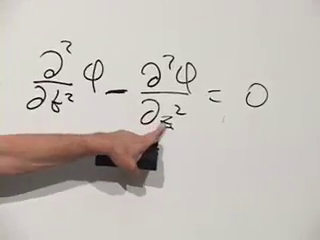
\includegraphics[width=0.56\textwidth]{lecture_58_figure_04.png}
\caption{Die eindimensionale skalare Wellengleichung als Modell für elektromagnetische Wellen.}
\lectureframe{00:47:03}
\end{figure}

Ihre allgemeine Form als Summe laufender Wellen lautet
\begin{equation}
\phi(z,t)=f(z-t)+g(z+t).
\end{equation}
Das Profil \(f(z-t)\) bewegt sich in Richtung zunehmender Werte von \(z\), denn ein Punkt konstanter Phase erfüllt \(z-t=\text{constant}\). Das Profil \(g(z+t)\) bewegt sich in die entgegengesetzte Richtung. Keines der Profile muss sinusförmig sein; jede hinreichend glatte Form verschiebt sich, ohne ihre Gestalt zu ändern.

Sinusfunktionen sind dennoch praktisch:
\begin{equation}
\phi(z,t)=A\cos\!\bigl(k(z-t)\bigr).
\end{equation}
Die Wellenzahl \(k\) bestimmt die Wellenlänge:
\begin{equation}
\lambda=\frac{2\pi}{k}.
\end{equation}
Ein großer Wert von \(k\) führt zu schnellen räumlichen Oszillationen und einer kurzen Wellenlänge; ein kleiner Wert von \(k\) führt zu einer langen Wellenlänge. Dieselben Profile werden bald zu Komponenten von \(\mathbf E\) und \(\mathbf B\).

\section{Die Vektorrechnung, die Maxwell braucht}

Die Maxwell-Gleichungen sind mit Skalarprodukten, Kreuzprodukten, Divergenz und Rotation formuliert. Es lohnt sich, die Notation einmal neu aufzubauen, denn bei den späteren Komponentenrechnungen verwenden wir genau diese Muster.

Für gewöhnliche Dreivektoren \(\mathbf a\) und \(\mathbf b\) ist das Skalarprodukt der Skalar
\begin{equation}
\mathbf a\cdot\mathbf b
=a_xb_x+a_yb_y+a_zb_z.
\end{equation}
Das Kreuzprodukt ist ein weiterer Vektor:
\begin{align}
(\mathbf a\times\mathbf b)_x&=a_yb_z-a_zb_y,\\
(\mathbf a\times\mathbf b)_y&=a_zb_x-a_xb_z,\\
(\mathbf a\times\mathbf b)_z&=a_xb_y-a_yb_x.
\end{align}
Die übrigen Komponenten ergeben sich aus der zyklischen Reihenfolge \(x\to y\to z\to x\).

Führen wir den Differentialoperator ein:
\begin{equation}
\boldsymbol\nabla=
\left(\partial_x,\partial_y,\partial_z\right).
\end{equation}
Seine Einträge sind Operatoren und keine gewöhnlichen Zahlen, doch die Muster für Skalar- und Kreuzprodukte lassen sich weiterhin verwenden. Für ein Vektorfeld \(\mathbf A\) ist
\begin{equation}
\boldsymbol\nabla\cdot\mathbf A
=\partial_xA_x+\partial_yA_y+\partial_zA_z
\label{eq:divergence}
\end{equation}
die Divergenz, während
\begin{align}
(\boldsymbol\nabla\times\mathbf A)_x
 &=\partial_yA_z-\partial_zA_y,\\
(\boldsymbol\nabla\times\mathbf A)_y
 &=\partial_zA_x-\partial_xA_z,\\
(\boldsymbol\nabla\times\mathbf A)_z
 &=\partial_xA_y-\partial_yA_x
\label{eq:curl}
\end{align}
die Komponenten der Rotation sind.

Die Geometrie ist ebenso wichtig wie die Formeln. Ein Vektorfeld hat dort eine positive Divergenz, wo es so aussieht, als ströme es von einer Quelle nach außen. Es hat dort eine Rotation, wo es umläuft. Das radiale elektrische Feld einer Punktladung veranschaulicht die Divergenz; das Magnetfeld, das sich um einen stromdurchflossenen Draht windet, veranschaulicht die Rotation. Ein räumlich konstantes Vektorfeld hat weder das eine noch das andere.

\section{Die Maxwell-Gleichungen im Vakuum}

In Abwesenheit von Ladung und Strom lauten die Maxwell-Gleichungen
\begin{align}
\boldsymbol\nabla\times\mathbf E&=-\partial_t\mathbf B,
\label{eq:faraday-vac}\\
\boldsymbol\nabla\cdot\mathbf B&=0,
\label{eq:gauss-b-vac}\\
\boldsymbol\nabla\times\mathbf B&=\partial_t\mathbf E,
\label{eq:ampere-vac}\\
\boldsymbol\nabla\cdot\mathbf E&=0.
\label{eq:gauss-e-vac}
\end{align}
Die beiden Rotationsgleichungen gehen nahezu ineinander über, wenn man \(\mathbf E\) und \(\mathbf B\) vertauscht; ein wesentliches Minuszeichen unterscheidet sie jedoch. Die beiden Divergenzgleichungen besagen, dass keines der Felder in dem betrachteten Vakuumbereich eine Quelle hat. Die Divergenz des Magnetfelds bleibt auch dann null, wenn elektrische Quellen wieder berücksichtigt werden; im gewöhnlichen Elektromagnetismus gibt es keine magnetische Ladung.

\begin{figure}[H]
\centering
\includegraphics[width=0.76\textwidth]{lecture_58_figure_06.png}
\caption{Die vier Maxwell-Gleichungen im Vakuum, so angeordnet, dass die weitgehende Symmetrie zwischen elektrischen und magnetischen Feldern sichtbar wird.}
\lectureframe{00:27:30}
\end{figure}

Die Ladungsdichte \(\rho\) wird später die Null auf der rechten Seite von Gleichung~\eqref{eq:gauss-e-vac} ersetzen, und die Stromdichte \(\mathbf J\) wird in Gleichung~\eqref{eq:ampere-vac} eingehen. Diese Terme lassen wir vorerst weg. Die quellenfreien Gleichungen zeigen die Transformationsstruktur und den Wellenmechanismus mit möglichst wenigen zusätzlichen Termen.

Sie schärfen auch Einsteins Rätsel. Ein Galilei-Beobachter, der einer Welle folgt, würde erwarten, Geschwindigkeiten voneinander abzuziehen und eine kleinere Wellengeschwindigkeit zu messen. Wenn jedoch dieselben Maxwell-Gleichungen in jedem Inertialsystem gelten, leitet jeder Beobachter daraus dieselbe Wellengeschwindigkeit von eins ab. Die Lösung besteht nicht darin, die Wellengleichung von einem Bezugssystem zum anderen abzuändern. Sie besteht darin, die Lorentz-Transformation zu verwenden und die Maxwell-Gleichungen in Größen darzustellen, deren Transformationsgesetze bereits bekannt sind.

\section{Elektrische und magnetische Felder als ein Tensor}

Die elektrischen und magnetischen Felder werden im antisymmetrischen Feldtensor zusammengefasst:
\begin{equation}
F^{\mu\nu}=
\begin{pmatrix}
0   & -E_x & -E_y & -E_z\\
E_x & 0    & -B_z & B_y\\
E_y & B_z  & 0    & -B_x\\
E_z & -B_y & B_x  & 0
\end{pmatrix},
\label{eq:l0203-field-tensor}
\end{equation}
wobei die Reihenfolge von Zeilen und Spalten \(t,x,y,z\) ist. Die Antisymmetrie
\begin{equation}
F^{\mu\nu}=-F^{\nu\mu},
\end{equation}
erzwingt, dass die Diagonaleinträge verschwinden, und bestimmt die untere Hälfte der Matrix durch die obere Hälfte. Die Raum-Zeit-Einträge enthalten \(\mathbf E\); die rein räumlichen Einträge enthalten \(\mathbf B\).

\begin{figure}[H]
\centering
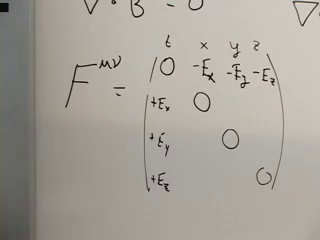
\includegraphics[width=0.58\textwidth]{lecture_58_figure_03.png}
\caption{Der vervollständigte elektromagnetische Feldtensor mit seinen elektrischen und magnetischen Einträgen.}
\lectureframe{00:32:05}
\end{figure}

Die Bedeutung von \(F^{\mu\nu}\) liegt nicht bloß darin, dass sich sechs Feldkomponenten in einer Matrix unterbringen lassen. Unter einer Lorentz-Transformation transformiert er sich wie ein Tensor zweiter Stufe. Von verschiedenen Beobachtern gemessene elektrische und magnetische Felder mischen sich daher genau so, wie es nötig ist, damit sich das gesamte Objekt konsistent transformiert.

Es gibt einen zweiten antisymmetrischen Tensor, den dualen Feldtensor \(\widetilde F^{\mu\nu}\). Gemäß der hier verwendeten Konvention erhält man ihn aus Gleichung~\eqref{eq:l0203-field-tensor} durch die Ersetzung
\begin{equation}
\mathbf E\longmapsto-\mathbf B,
\qquad
\mathbf B\longmapsto\mathbf E.
\label{eq:dual-replacement}
\end{equation}
Damit gilt
\begin{equation}
\widetilde F^{\mu\nu}=
\begin{pmatrix}
0    & B_x  & B_y  & B_z\\
-B_x & 0    & -E_z & E_y\\
-B_y & E_z  & 0    & -E_x\\
-B_z & -E_y & E_x  & 0
\end{pmatrix}.
\label{eq:dual-tensor}
\end{equation}
Das Vorzeichen in Gleichung~\eqref{eq:dual-replacement} ist wichtig. In der Vorlesung wird zunächst ein mündlicher Austausch versucht, dann die Abweichung beim Vorzeichen bemerkt und korrigiert, bevor die Matrix vervollständigt wird.

\begin{figure}[H]
\centering
\includegraphics[width=0.58\textwidth]{lecture_58_figure_07.png}
\caption{Der duale Tensor entsteht durch den Austausch der elektrischen und magnetischen Einträge mit dem erforderlichen Vorzeichen.}
\lectureframe{00:35:45}
\end{figure}

\section{Die kovarianten Gleichungen im Vakuum}

Jede Maxwell-Gleichung enthält eine Ableitung. Verknüpft man einen Rang-zwei-Tensor mit einer Ableitung, bleibt ein Index frei. Die natürlichen kovarianten Gleichungen sind daher
\begin{align}
\partial_\mu F^{\mu\nu}&=0,
\label{eq:maxwell-covariant-vac}\\
\partial_\mu\widetilde F^{\mu\nu}&=0.
\label{eq:maxwell-dual-vac}
\end{align}
Für jeden festen Wert von \(\nu\) ist Gleichung~\eqref{eq:maxwell-covariant-vac} eine Gleichung. Da \(\nu\) die Werte \(t,x,y,z\) annehmen kann, umfasst sie vier skalare Gleichungen. Gleichung~\eqref{eq:maxwell-dual-vac} umfasst die übrigen vier. Das entspricht den beiden Vektor-Rotationsgleichungen und den beiden skalaren Divergenzgleichungen der ursprünglichen Liste.

Die Kurzschreibweise ist nur dann nützlich, wenn sie die vertrauten Gleichungen wiedergibt. Setzen wir \(\nu=z\):
\begin{align}
\partial_\mu F^{\mu z}
&=\partial_tF^{tz}
  +\partial_xF^{xz}
  +\partial_yF^{yz}
  +\partial_zF^{zz}\\
&=-\partial_tE_z+\partial_xB_y-\partial_yB_x\\
&=-\partial_tE_z+
  \bigl(\boldsymbol\nabla\times\mathbf B\bigr)_z.
\end{align}
Der Term \(F^{zz}\) verschwindet aufgrund der Antisymmetrie. Setzt man den Ausdruck gleich null, erhält man die \(z\)-Komponente von
\begin{equation}
\boldsymbol\nabla\times\mathbf B=\partial_t\mathbf E.
\end{equation}
Die \(x\)- und \(y\)-Komponenten ergeben sich durch zyklisches Vertauschen der Indizes.

\begin{figure}[H]
\centering
\includegraphics[width=0.76\textwidth]{lecture_58_figure_08.png}
\caption{Komponentenweise Entwicklung der kovarianten Feldgleichung: Der diagonale Tensoreintrag verschwindet, und die übrigen Terme ergeben wieder die Maxwell-Gleichungen.}
\lectureframe{00:43:30}
\end{figure}

Betrachten wir nun die Zeitkomponente:
\begin{align}
\partial_\mu F^{\mu t}
&=\partial_tF^{tt}
  +\partial_xF^{xt}
  +\partial_yF^{yt}
  +\partial_zF^{zt}\\
&=\partial_xE_x+\partial_yE_y+\partial_zE_z\\
&=\boldsymbol\nabla\cdot\mathbf E.
\end{align}
Damit ergibt sich Gleichung~\eqref{eq:gauss-e-vac}. Dieselben Überprüfungen für den dualen Tensor liefern
\(\boldsymbol\nabla\cdot\mathbf B=0\) und
\(\boldsymbol\nabla\times\mathbf E=-\partial_t\mathbf B\).

Damit sind die kompakten Gleichungen hergeleitet und nicht bloß vermutet. Ihre Struktur mit einem freien Index zeigt, dass es Vierergleichungen sind; eine Lorentz-Transformation ändert also ihre Komponenten, aber nicht ihre Form. Das ist die präzise Bedeutung der Aussage, dass die Maxwell-Gleichungen im Vakuum in jedem Inertialsystem dieselben sind.

\section{Von Gleichungen erster Ordnung zur Welle}

Die Maxwell-Gleichungen enthalten nur Ableitungen erster Ordnung, während eine Wellengleichung Ableitungen zweiter Ordnung enthält. Der scheinbare Widerspruch löst sich dadurch auf, dass die Maxwell-Theorie zwei Felder miteinander koppelt. Ein Paar von Gleichungen erster Ordnung für \(\mathbf E\) und \(\mathbf B\) lässt sich zu einer Gleichung zweiter Ordnung für jeweils eines der beiden Felder allein zusammenfassen.

Leiten wir Gleichung~\eqref{eq:ampere-vac} nach der Zeit ab:
\begin{equation}
\partial_t^2\mathbf E
=\boldsymbol\nabla\times\partial_t\mathbf B.
\end{equation}
Das Faraday-Gesetz liefert die Zeitableitung von \(\mathbf B\):
\begin{equation}
\partial_t\mathbf B=-\boldsymbol\nabla\times\mathbf E,
\end{equation}
und damit
\begin{equation}
\partial_t^2\mathbf E
=-\boldsymbol\nabla\times
  \bigl(\boldsymbol\nabla\times\mathbf E\bigr).
\label{eq:double-curl}
\end{equation}

Auf der Tafel wird eine Komponente durchgerechnet, statt eine auswendig gelernte Identität zu verwenden. Für die \(x\)-Komponente gilt
\begin{align}
\bigl[\boldsymbol\nabla\times
(\boldsymbol\nabla\times\mathbf E)\bigr]_x
&=\partial_y(\boldsymbol\nabla\times\mathbf E)_z
 -\partial_z(\boldsymbol\nabla\times\mathbf E)_y\\
&=\partial_y(\partial_xE_y-\partial_yE_x)\\
&\quad-\partial_z(\partial_zE_x-\partial_xE_z)\\
&=\partial_x(\partial_yE_y+\partial_zE_z)
 -\partial_y^2E_x\\
&\quad-\partial_z^2E_x.
\end{align}
Addieren und subtrahieren wir \(\partial_x^2E_x\), um die Divergenz sichtbar zu machen:
\begin{align}
\bigl[\boldsymbol\nabla\times
(\boldsymbol\nabla\times\mathbf E)\bigr]_x
&=\partial_x(\boldsymbol\nabla\cdot\mathbf E)
 -\nabla^2E_x.
\label{eq:double-curl-x}
\end{align}
Im Vakuum gilt \(\boldsymbol\nabla\cdot\mathbf E=0\). Aus den Gleichungen~\eqref{eq:double-curl} und \eqref{eq:double-curl-x} folgt
\begin{equation}
\left(\partial_t^2-\nabla^2\right)E_x=0.
\label{eq:ex-wave}
\end{equation}

\begin{figure}[H]
\centering
\includegraphics[width=0.72\textwidth]{lecture_58_figure_09.png}
\caption{Die Komponentenrechnung führt zur Wellengleichung für \(E_x\).}
\lectureframe{00:57:10}
\end{figure}

Dieselbe Rechnung gilt für \(E_y\) und \(E_z\); eine analoge Elimination ergibt
\begin{equation}
\left(\partial_t^2-\nabla^2\right)\mathbf B=0.
\end{equation}
Elektrische und magnetische Felder können sich folglich als Wellen durch den leeren Raum ausbreiten. In den hier verwendeten Einheiten beträgt ihre Geschwindigkeit eins; stellt man die üblichen Einheiten wieder her, ist sie gleich \(c\).

\section{Eine ebene Welle und ihre Polarisation}

Konstruieren wir eine einfache Welle, die sich in positiver \(z\)-Richtung ausbreitet:
\begin{equation}
\mathbf E(z,t)
=\widehat{\mathbf x}\,E_0
  \cos\!\bigl(k(z-t)\bigr).
\label{eq:plane-e}
\end{equation}
Ihr Profil bewegt sich entlang \(z\), ohne seine Form zu ändern. Da das elektrische Feld entlang der \(x\)-Achse zeigt, ist die Welle in \(x\)-Richtung linear polarisiert. Wir haben \(E_y=0\) gewählt, um das Beispiel einfach zu halten; eine zweite transversale Polarisation ließe sich ergänzen.

Die longitudinale Komponente ist nicht ebenso frei. Da die Welle nur von \(z\) und \(t\) abhängt, gilt
\begin{equation}
\boldsymbol\nabla\cdot\mathbf E
=\partial_zE_z=0.
\end{equation}
Somit kann \(E_z\) konstant sein, aber nicht das veränderliche Wellenprofil enthalten. Ein homogenes Hintergrundfeld kann unabhängig davon überlagert oder entfernt werden; es gehört nicht zur sich ausbreitenden Strahlung. Die Welle selbst ist transversal:
\begin{equation}
\mathbf E_{\mathrm{wave}}\cdot\widehat{\mathbf z}=0.
\end{equation}

Das Faraday-Gesetz legt das Magnetfeld fest. Für Gleichung~\eqref{eq:plane-e} ist die einzige von null verschiedene Komponente von \(\boldsymbol\nabla\times\mathbf E\) die \(y\)-Komponente:
\begin{equation}
(\boldsymbol\nabla\times\mathbf E)_y=\partial_zE_x.
\end{equation}
Folglich zeigt \(\partial_t\mathbf B\) in Richtung \(y\), und eine dazu passende Wahl ist
\begin{equation}
\mathbf B(z,t)
=\widehat{\mathbf y}\,E_0
  \cos\!\bigl(k(z-t)\bigr).
\label{eq:plane-b}
\end{equation}
In diesen Einheiten sind die Amplituden der elektrischen und magnetischen Felder gleich. Ihre Orientierung erfüllt
\begin{equation}
\mathbf E\perp\mathbf B,
\qquad
\mathbf E\perp\widehat{\mathbf z},
\qquad
\mathbf B\perp\widehat{\mathbf z},
\qquad
\mathbf E\times\mathbf B\parallel\widehat{\mathbf z}.
\end{equation}

\begin{figure}[H]
\centering
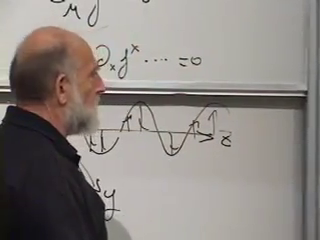
\includegraphics[width=0.70\textwidth]{lecture_58_figure_05.png}
\caption{Die fertige Skizze der transversalen elektromagnetischen Welle auf der Tafel: Die elektrischen und magnetischen Oszillationen stehen senkrecht zueinander und zur Ausbreitungsrichtung.}
\lectureframe{01:05:25}
\end{figure}

\begin{figure}[H]
\centering
\scalebox{0.90}{%
\begin{tikzpicture}[x=1cm,y=1cm,>=Latex]
  \draw[->,thick] (0,0) -- (8.2,0) node[right] {$z$};
  \draw[->,thick] (0,-1.6) -- (0,1.7) node[above] {$x$};
  \draw[->,thick] (0,0) -- (-1.15,-0.8) node[below left] {$y$};
  \draw[blue!70!black,thick,domain=0:7.5,samples=120]
    plot (\x,{0.95*sin(90*\x)});
  \foreach \z/\s in {0.8/1,2.8/-1,4.8/1,6.8/-1}{
    \draw[->,green!45!black,thick]
      (\z,0) -- ++({-0.55*\s},{-0.38*\s});
  }
  \node[blue!70!black] at (6.9,1.25) {$\mathbf E$};
  \node[green!45!black] at (5.2,-1.05) {$\mathbf B$};
  \draw[->,very thick] (6.2,1.55) -- (7.7,1.55)
    node[midway,above] {propagation};
\end{tikzpicture}
}
\caption{Die Felder \(\mathbf E\) und \(\mathbf B\) stehen senkrecht zueinander und zur Ausbreitungsrichtung.}
\end{figure}

Das ist die typische Eigenschaft des Lichts und aller elektromagnetischen Strahlung im Vakuum. Da die Gleichungen, aus denen die Welle folgt, Lorentz-kovariant sind, beschreibt auch ein anderer Inertialbeobachter eine elektromagnetische Welle, die sich mit \(c\) ausbreitet und transversale elektrische und magnetische Felder besitzt.

\section{Ladungsdichte und Stromdichte}

Nun führen wir die Quellen wieder ein, die wir vorübergehend beiseitegelassen haben. Befinden sich viele geladene Teilchen in einem Gebiet, ist es nützlich, sie durch Mittelung zu einer kontinuierlichen Ladungsdichte zusammenzufassen:
\begin{equation}
\rho(\mathbf x,t)=\frac{dQ}{dV}.
\end{equation}
Diese Näherung ähnelt der Beschreibung von Wasser als kontinuierlicher Flüssigkeit, obwohl es aus Molekülen besteht. Positive und negative Ladungen gehen mit entgegengesetzten Vorzeichen ein, sodass \(\rho\) die Nettoladung pro Volumeneinheit ist.

Die Ladung in einem gewählten Gebiet \(V\) beträgt
\begin{equation}
Q_V(t)=\int_V\rho(\mathbf x,t)\,dV.
\label{eq:charge-volume}
\end{equation}
Die Dichte kann von Ort und Zeit abhängen. Eine Ansammlung von Ladung kann sich von einem Punkt entfernen und dort die lokale Dichte ändern. Sie kann sich jedoch nicht beliebig ändern. Die Natur erhält die elektrische Ladung.

Die globale Erhaltung allein wäre zu schwach. Sie würde zulassen, dass Ladung auf der Erde verschwindet und im selben Augenblick auf dem Mars wieder auftaucht, solange die Gesamtladung unverändert bliebe. Die stärkere Aussage gilt lokal: Ladung kann einen Ort nur verlassen und einen anderen erreichen, indem sie durch den dazwischenliegenden Raum strömt.

Um diese Strömung zu beschreiben, betrachten wir ein infinitesimales orientiertes Flächenelement:
\begin{equation}
d\boldsymbol\sigma=\widehat{\mathbf n}\,d\sigma.
\end{equation}
Sein Betrag ist die Fläche, seine Richtung steht senkrecht auf der Fläche. Die Stromdichte \(\mathbf J\) ist so definiert, dass die Ladung, die das Flächenelement pro Zeit durchquert, gleich
\begin{equation}
\frac{dQ}{dt}=\mathbf J\cdot d\boldsymbol\sigma.
\label{eq:current-flux-element}
\end{equation}
ist. Der Betrag von \(\mathbf J\) entspricht der Ladung pro Flächeneinheit und Zeit; seine Richtung ist die des Flusses positiver Ladung.

\begin{figure}[H]
\centering
\includegraphics[width=0.64\textwidth]{lecture_58_figure_10.png}
\caption{Ein orientiertes Flächenelement und der Flussfaktor \(d\boldsymbol\sigma\cdot\mathbf J\).}
\lectureframe{01:18:15}
\end{figure}

Das Skalarprodukt wählt die Komponente senkrecht zur Fläche aus. Ein tangential zur Fläche verlaufender Strom durchquert keine der beiden Seiten und trägt null bei. Ein Strom parallel zur Flächennormalen hat bei festem Betrag den maximalen Fluss. Ein Drahtstrom ist ein Sonderfall, doch \(\mathbf J\) kann auch einen Ladungsfluss durch eine Fläche oder durch den dreidimensionalen Raum beschreiben.

\section{Lokale Erhaltung und die Kontinuitätsgleichung}

Wir betrachten ein festes Gebiet \(V\) im Raum und richten jedes Element seines geschlossenen Randes \(\partial V\) nach außen aus. Gibt es einen nach außen gerichteten Nettostrom, nimmt die Ladung im Inneren ab:
\begin{equation}
\frac{dQ_V}{dt}
=-\oint_{\partial V}\mathbf J\cdot d\boldsymbol\sigma.
\label{eq:integral-conservation}
\end{equation}
Das Minuszeichen ist physikalisch bedingt und keine Konvention: Ein positiver nach außen gerichteter Fluss entfernt positive Ladung aus dem Gebiet. Mit Gleichung~\eqref{eq:charge-volume} folgt
\begin{equation}
\int_V\partial_t\rho\,dV
=-\oint_{\partial V}\mathbf J\cdot d\boldsymbol\sigma.
\label{eq:integral-continuity-one}
\end{equation}

\begin{figure}[H]
\centering
\includegraphics[width=0.72\textwidth]{lecture_58_figure_11.png}
\caption{Das Erhaltungsgesetz für ein festes Gebiet, nachdem der Fluss durch die Oberfläche in eine Volumenaussage umgewandelt wurde.}
\lectureframe{01:29:00}
\end{figure}

Der Satz von Gauß, auch Divergenzsatz genannt, setzt den Fluss durch eine geschlossene Fläche mit der Divergenz in ihrem Inneren in Beziehung:
\begin{equation}
\oint_{\partial V}\mathbf A\cdot d\boldsymbol\sigma
=\int_V\boldsymbol\nabla\cdot\mathbf A\,dV.
\label{eq:divergence-theorem}
\end{equation}
Man kann sich verborgene Rohre vorstellen, die an verschiedenen Stellen im Inneren eines Gefäßes Wasser einspeisen. Die Divergenz misst die lokale Rate, mit der Wasser an den Rohrenden austritt; das Flächenintegral misst die gesamte Wassermenge, die das Gefäß verlässt. Was im Inneren als nach außen gerichtete Strömung entsteht, muss schließlich die Begrenzungsfläche durchqueren.

Wenden wir Gleichung~\eqref{eq:divergence-theorem} auf \(\mathbf J\) an, erhalten wir
\begin{equation}
\int_V
\left(\partial_t\rho+\boldsymbol\nabla\cdot\mathbf J\right)dV=0.
\end{equation}
Diese Beziehung gilt für jedes mögliche Gebiet \(V\). Daher muss der Integrand an jedem Punkt verschwinden:
\begin{equation}
\boxed{\partial_t\rho+\boldsymbol\nabla\cdot\mathbf J=0.}
\label{eq:continuity-three}
\end{equation}

\begin{figure}[H]
\centering
\includegraphics[width=0.72\textwidth]{lecture_58_figure_12.png}
\caption{Die lokale Kontinuitätsgleichung, komponentenweise ausgeschrieben.}
\lectureframe{01:29:50}
\end{figure}

Gleichung~\eqref{eq:continuity-three} besagt genau, was die lokale Erhaltung verlangt. Nimmt die Ladungsdichte an einem Punkt oder in einem kleinen Gebiet ab, muss der Strom von dort nach außen divergieren. Konvergiert der Strom nach innen, nimmt die Ladungsdichte zu.

Dichte und Strom bilden auf natürliche Weise den Viererstrom
\begin{equation}
J^\mu=(\rho,J_x,J_y,J_z)
\label{eq:four-current}
\end{equation}
in Einheiten, in denen \(c=1\) gilt. Die Kontinuitätsgleichung wird zur Lorentz-Skalargleichung
\begin{equation}
\partial_\mu J^\mu=0.
\label{eq:continuity-four}
\end{equation}
Der Fluss einer relativistischen Verteilung sollte sich wie ein Vierervektor transformieren, ebenso wie die Vierergeschwindigkeit eines einzelnen Teilchens. Gleichung~\eqref{eq:continuity-four} gewährleistet die lokale Ladungserhaltung in jedem Inertialsystem.

\section{Die Maxwell-Gleichungen mit Quellen}

Mit Ladung und Strom lauten die Gleichungen
\begin{align}
\boldsymbol\nabla\cdot\mathbf E&=\rho,
\label{eq:gauss-e-source}\\
\boldsymbol\nabla\cdot\mathbf B&=0,\\
\boldsymbol\nabla\times\mathbf E&=-\partial_t\mathbf B,\\
\boldsymbol\nabla\times\mathbf B&=\partial_t\mathbf E+\mathbf J.
\label{eq:ampere-source}
\end{align}
Die Gleichungen mit elektrischen Quellen lassen sich zusammenfassen zu
\begin{equation}
\boxed{\partial_\mu F^{\mu\nu}=J^\nu,}
\label{eq:maxwell-source-covariant}
\end{equation}
während das quellenfreie magnetische Gleichungspaar unverändert bleibt:
\begin{equation}
\boxed{\partial_\mu\widetilde F^{\mu\nu}=0.}
\label{eq:maxwell-dual-source}
\end{equation}

\begin{figure}[H]
\centering
\includegraphics[width=0.78\textwidth]{lecture_58_figure_13.png}
\caption{Die Maxwell-Gleichungen mit Quellen neben ihrer kovarianten Form \(\partial_\mu F^{\mu\nu}=J^\nu\).}
\lectureframe{01:34:00}
\end{figure}

Die Zeitkomponente von Gleichung~\eqref{eq:maxwell-source-covariant} lautet
\begin{equation}
\partial_\mu F^{\mu t}=J^t=\rho,
\end{equation}
und die bereits durchgeführte Komponentenrechnung ergibt für ihre linke Seite
\(\boldsymbol\nabla\cdot\mathbf E\). Die drei räumlichen Komponenten reproduzieren
\(\boldsymbol\nabla\times\mathbf B=\partial_t\mathbf E+\mathbf J\).

Es gibt auch eine nützliche Konsistenzprüfung. Wenden wir \(\partial_\nu\) auf Gleichung~\eqref{eq:maxwell-source-covariant} an, erhalten wir
\begin{equation}
\partial_\nu J^\nu
=\partial_\nu\partial_\mu F^{\mu\nu}=0,
\end{equation}
denn die beiden Ableitungen sind unter \(\mu\leftrightarrow\nu\) symmetrisch, während \(F^{\mu\nu}\) antisymmetrisch ist.\editorialnote{Diese kurze Konsistenzprüfung folgt aus der kovarianten Gleichung und zeigt ausdrücklich, weshalb die Maxwell-Gleichungen mit Quellen automatisch die Kontinuitätsgleichung erfüllen.}

Damit ist die wechselseitige Struktur vollständig. Das Tensorkraftgesetz
\(f^\mu=qF^\mu{}_\nu u^\nu\)
beschreibt, wie Felder auf Ladungen wirken, und Gleichung~\eqref{eq:maxwell-source-covariant} beschreibt, wie Ladung und Strom Felder erzeugen. Beide sind Tensorgleichungen. Im Vakuum ergeben dieselben Feldgleichungen transversale Wellen, die sich mit \(c\) ausbreiten. Die Lorentz-Kovarianz und die elektromagnetische Wellengleichung treffen somit an dem Punkt zusammen, der den Ausgangspunkt der Herleitung bildete: Jeder Inertialbeobachter erhält dieselben Gesetze des Elektromagnetismus und dieselbe Lichtgeschwindigkeit.
